\documentclass{beamer}

\usefonttheme{professionalfonts} % using non standard fonts for beamer
\usefonttheme{serif} % default family is serif

%\usepackage{hyperref}

%\usepackage{minted}

\usepackage{animate}

\usepackage{graphicx}

\def\Put(#1,#2)#3{\leavevmode\makebox(0,0){\put(#1,#2){#3}}}

\usepackage{color}

\usepackage{tikz}

\usepackage{amssymb}

\usepackage{enumerate}


\newcommand\blfootnote[1]{%

  \begingroup

  \renewcommand\thefootnote{}\footnote{#1}%

  \addtocounter{footnote}{-1}%

  \endgroup

}

\makeatletter

%%%%%%%%%%%%%%%%%%%%%%%%%%%%%% Textclass specific LaTeX commands.

 % this default might be overridden by plain title style

 \newcommand\makebeamertitle{\frame{\maketitle}}%

 % (ERT) argument for the TOC

 \AtBeginDocument{%

   \let\origtableofcontents=\tableofcontents

   \def\tableofcontents{\@ifnextchar[{\origtableofcontents}{\gobbletableofcontents}}

   \def\gobbletableofcontents#1{\origtableofcontents}

 }

%%%%%%%%%%%%%%%%%%%%%%%%%%%%%% User specified LaTeX commands.

\usetheme{Malmoe}

% or ...

\useoutertheme{infolines}

\addtobeamertemplate{headline}{}{\vskip2pt}



\setbeamercovered{transparent}

% or whatever (possibly just delete it)

\makeatother

\begin{document}
\title[SDCEL report]{Geoinformatica paper extension}
\author[AC]{}
\institute[UCR]{University of California, Riverside}
\makebeamertitle
\newif\iflattersubsect

% \AtBeginSection[] {
%   \begin{frame}<beamer>
%     \frametitle{Outline} 
%     \tableofcontents[currentsection]  
%   \end{frame}
%   \lattersubsectfalse
% }

\AtBeginSubsection[] {
  \begin{frame}<beamer>
    \frametitle{Outline} 
    \tableofcontents[currentsubsection]  
  \end{frame}
}

\begin{frame}{So far...}
  \begin{itemize}
    \item Explore a couple of implementation of k-d tree as new data structure during partitioning:
      \begin{itemize}
        \item Brown's balanced K-d tree [\url{https://arxiv.org/abs/1410.5420}]
        \item Sedona's KDB tree [https://sedona.apache.org/]
      \end{itemize}
  \end{itemize}
\end{frame}

\begin{frame}{So far...}
  \begin{itemize}
    \item We had a serious concern about data availability during k-d construction to complete the optimization...
    \begin{itemize}
      \item At that stage we deal with a sample of the data.
      \item Not certain if we could even detect possible unbalanced cells.
    \end{itemize}
    \item but...
  \end{itemize}
\end{frame}

\begin{frame}{So far...}
  \begin{itemize}
    \item We had seen that given a representative sample detecting unbalanced cells is possible (maybe missing a few).
    \item During kd-tree creation we could compute a set of initial intervals.
    \item During edge partitioning we could update those interval accordingly (in progress).
    \item So, we could expect to save time for sorting and interval finding we perform later in the original approach.
  \end{itemize}
\end{frame}

\begin{frame}{Some questions about other comments...}
  \centering 
  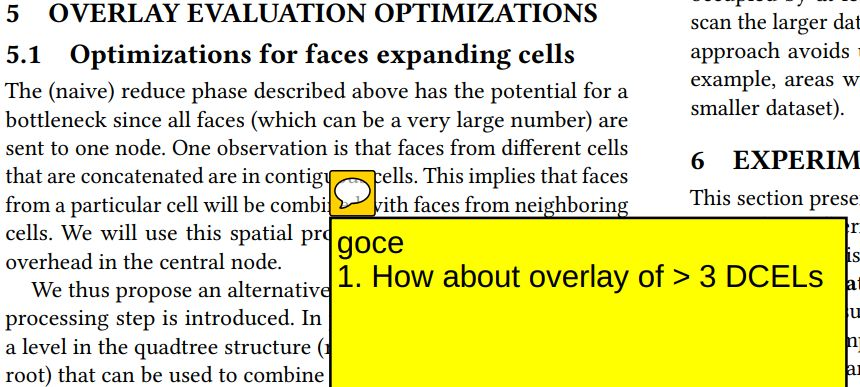
\includegraphics[width=0.6\textwidth]{figures/Q1}
  \begin{itemize}
    \item Is it more related to compute more than two layers at the same time or something like cascading?
  \end{itemize}
\end{frame}

\begin{frame}{Some questions about other comments...}
  \centering 
  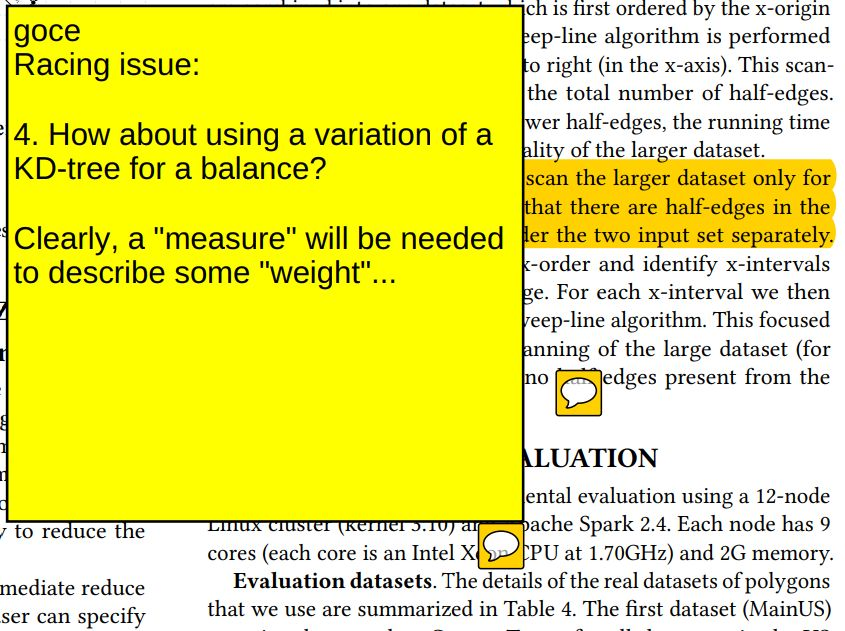
\includegraphics[width=0.5\textwidth]{figures/Q2}
  \begin{itemize}
    \item With a balanced data structure would we expect a more fair evaluation when we test different levels of the tree?
  \end{itemize}
\end{frame}

%\begin{frame}{Some invalids polygons...}
%    \centering 
    %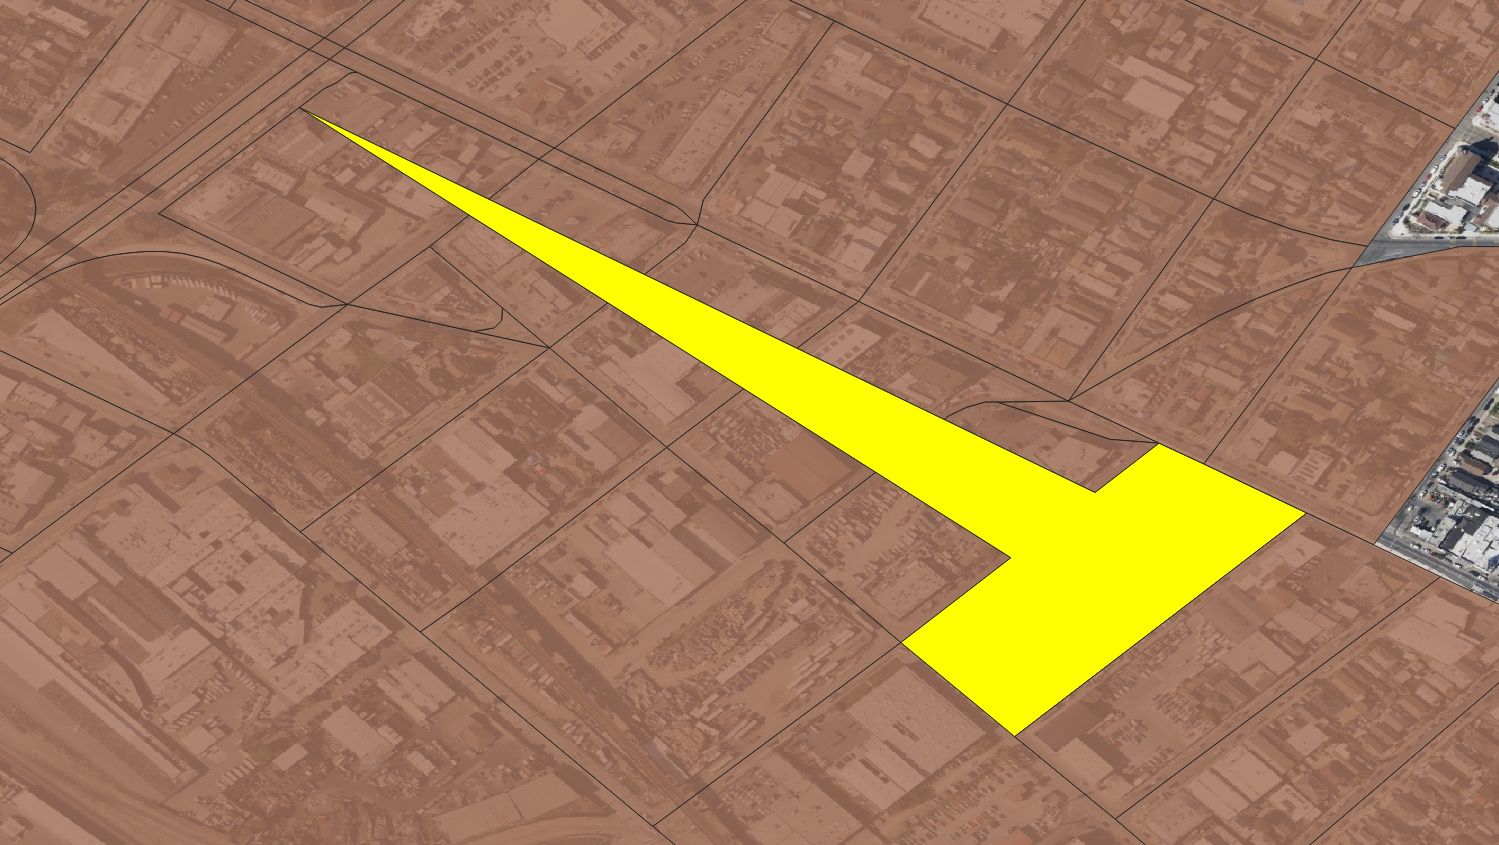
\includegraphics[width=0.8\textwidth]{figures/artifact02}
%\end{frame}

\end{document}
